本项目中全面运用了模块化的设计思想。在最初设计时(见图\ref{fig:design_architecture}),我们为项目设计了六个功能模块(键盘译码、渲染控制、UART发送与接受、VGA信号发生与处理)和一个调试模块。然而,终端本身功能的特点,即其事实上不对用户指令进行任何除译码外的处理,决定了其实这个系统中存在两条独立的信号通路,即:键盘输入→按键译码→UART发送,UART接收→指令处理→渲染→VGA输出。因此,在最终实现中(如图\ref{fig:final_architecture}),我们将项目分成了两个大模块,即键盘控制器\texttt{KeyboardController}与图形控制器\texttt{VideoController},二者分别处理上述的两条信号通路,完成各自的功能,互相独立。事实证明,这种解耦合的思想为我们的开发带来了很多的便利。

值得一提的是,本项目全部采用\texttt{SystemVerilog}进行编写。它带来了多个方便的新特性,如:
\begin{description}
  \item[\texttt{logic}类型] 整合了 \texttt{wire} 和 \texttt{reg} 类型,自动推导几类寄存器模型,减少无谓的区分。
  \item[\texttt{always\_comb, always\_latch, always\_ff}块] 可明确指定需要的逻辑类型(纯组合逻辑、锁存器、触发器),防止出现非预期电路和行为。
  \item[\texttt{struct}类型] 与C语言类似,可将一组值/信号进行单独赋值、统一绑定与传递。
  \item[\texttt{enum}类型] 与C语言类似,可以给常量赋名称,并有作用域限制,在状态机的设计中减少了出错的可能。
  \item[\texttt{typedef}关键字] 与C语言类似,可以给复杂的变量类型赋予别名,更直观好记。
  \item[\texttt{define, generate}关键字] 可以方便地在预处理阶段批量生成代码,以及在综合阶段批量生成元件,适合大量小元器件并行使用的场合。
\end{description}

进一步地,\texttt{SystemVerilog}在电路的测试验证中具有 \texttt{VHDL} 与 \texttt{Verilog}不可比拟的灵活性、便捷性。我们强烈建议各位学习这门先进的硬件描述语言,也建议老师在今后的教学中考虑采纳它,与现代VLSI设计接轨。

\begin{figure}[htbp]
\centerline{
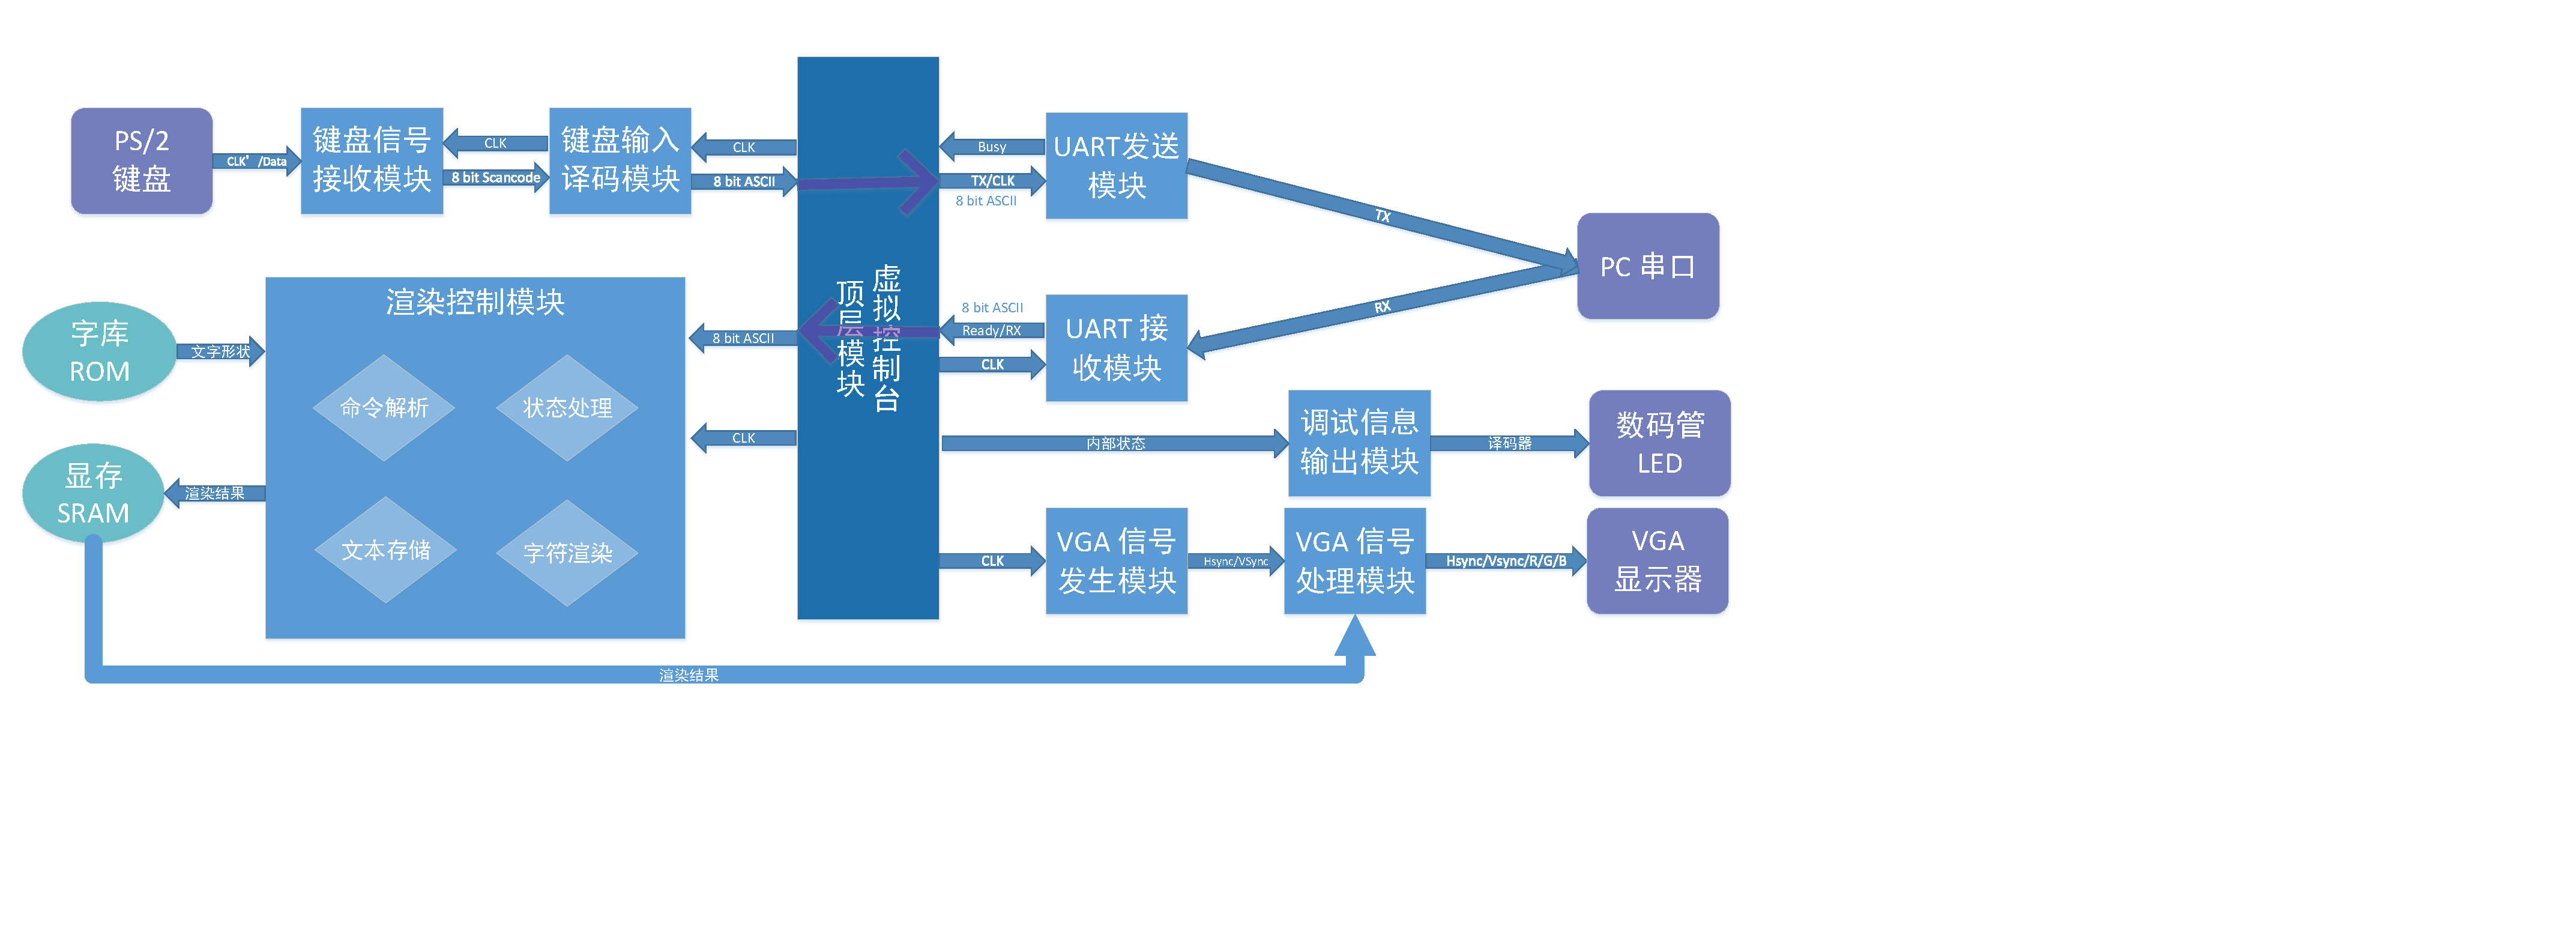
\includegraphics[width=0.95\paperwidth]{architecture_design_visio.pdf}
}
\label{fig:design_architecture}
\caption{项目设计架构}
\end{figure}

\begin{figure}[htbp]
\centerline{
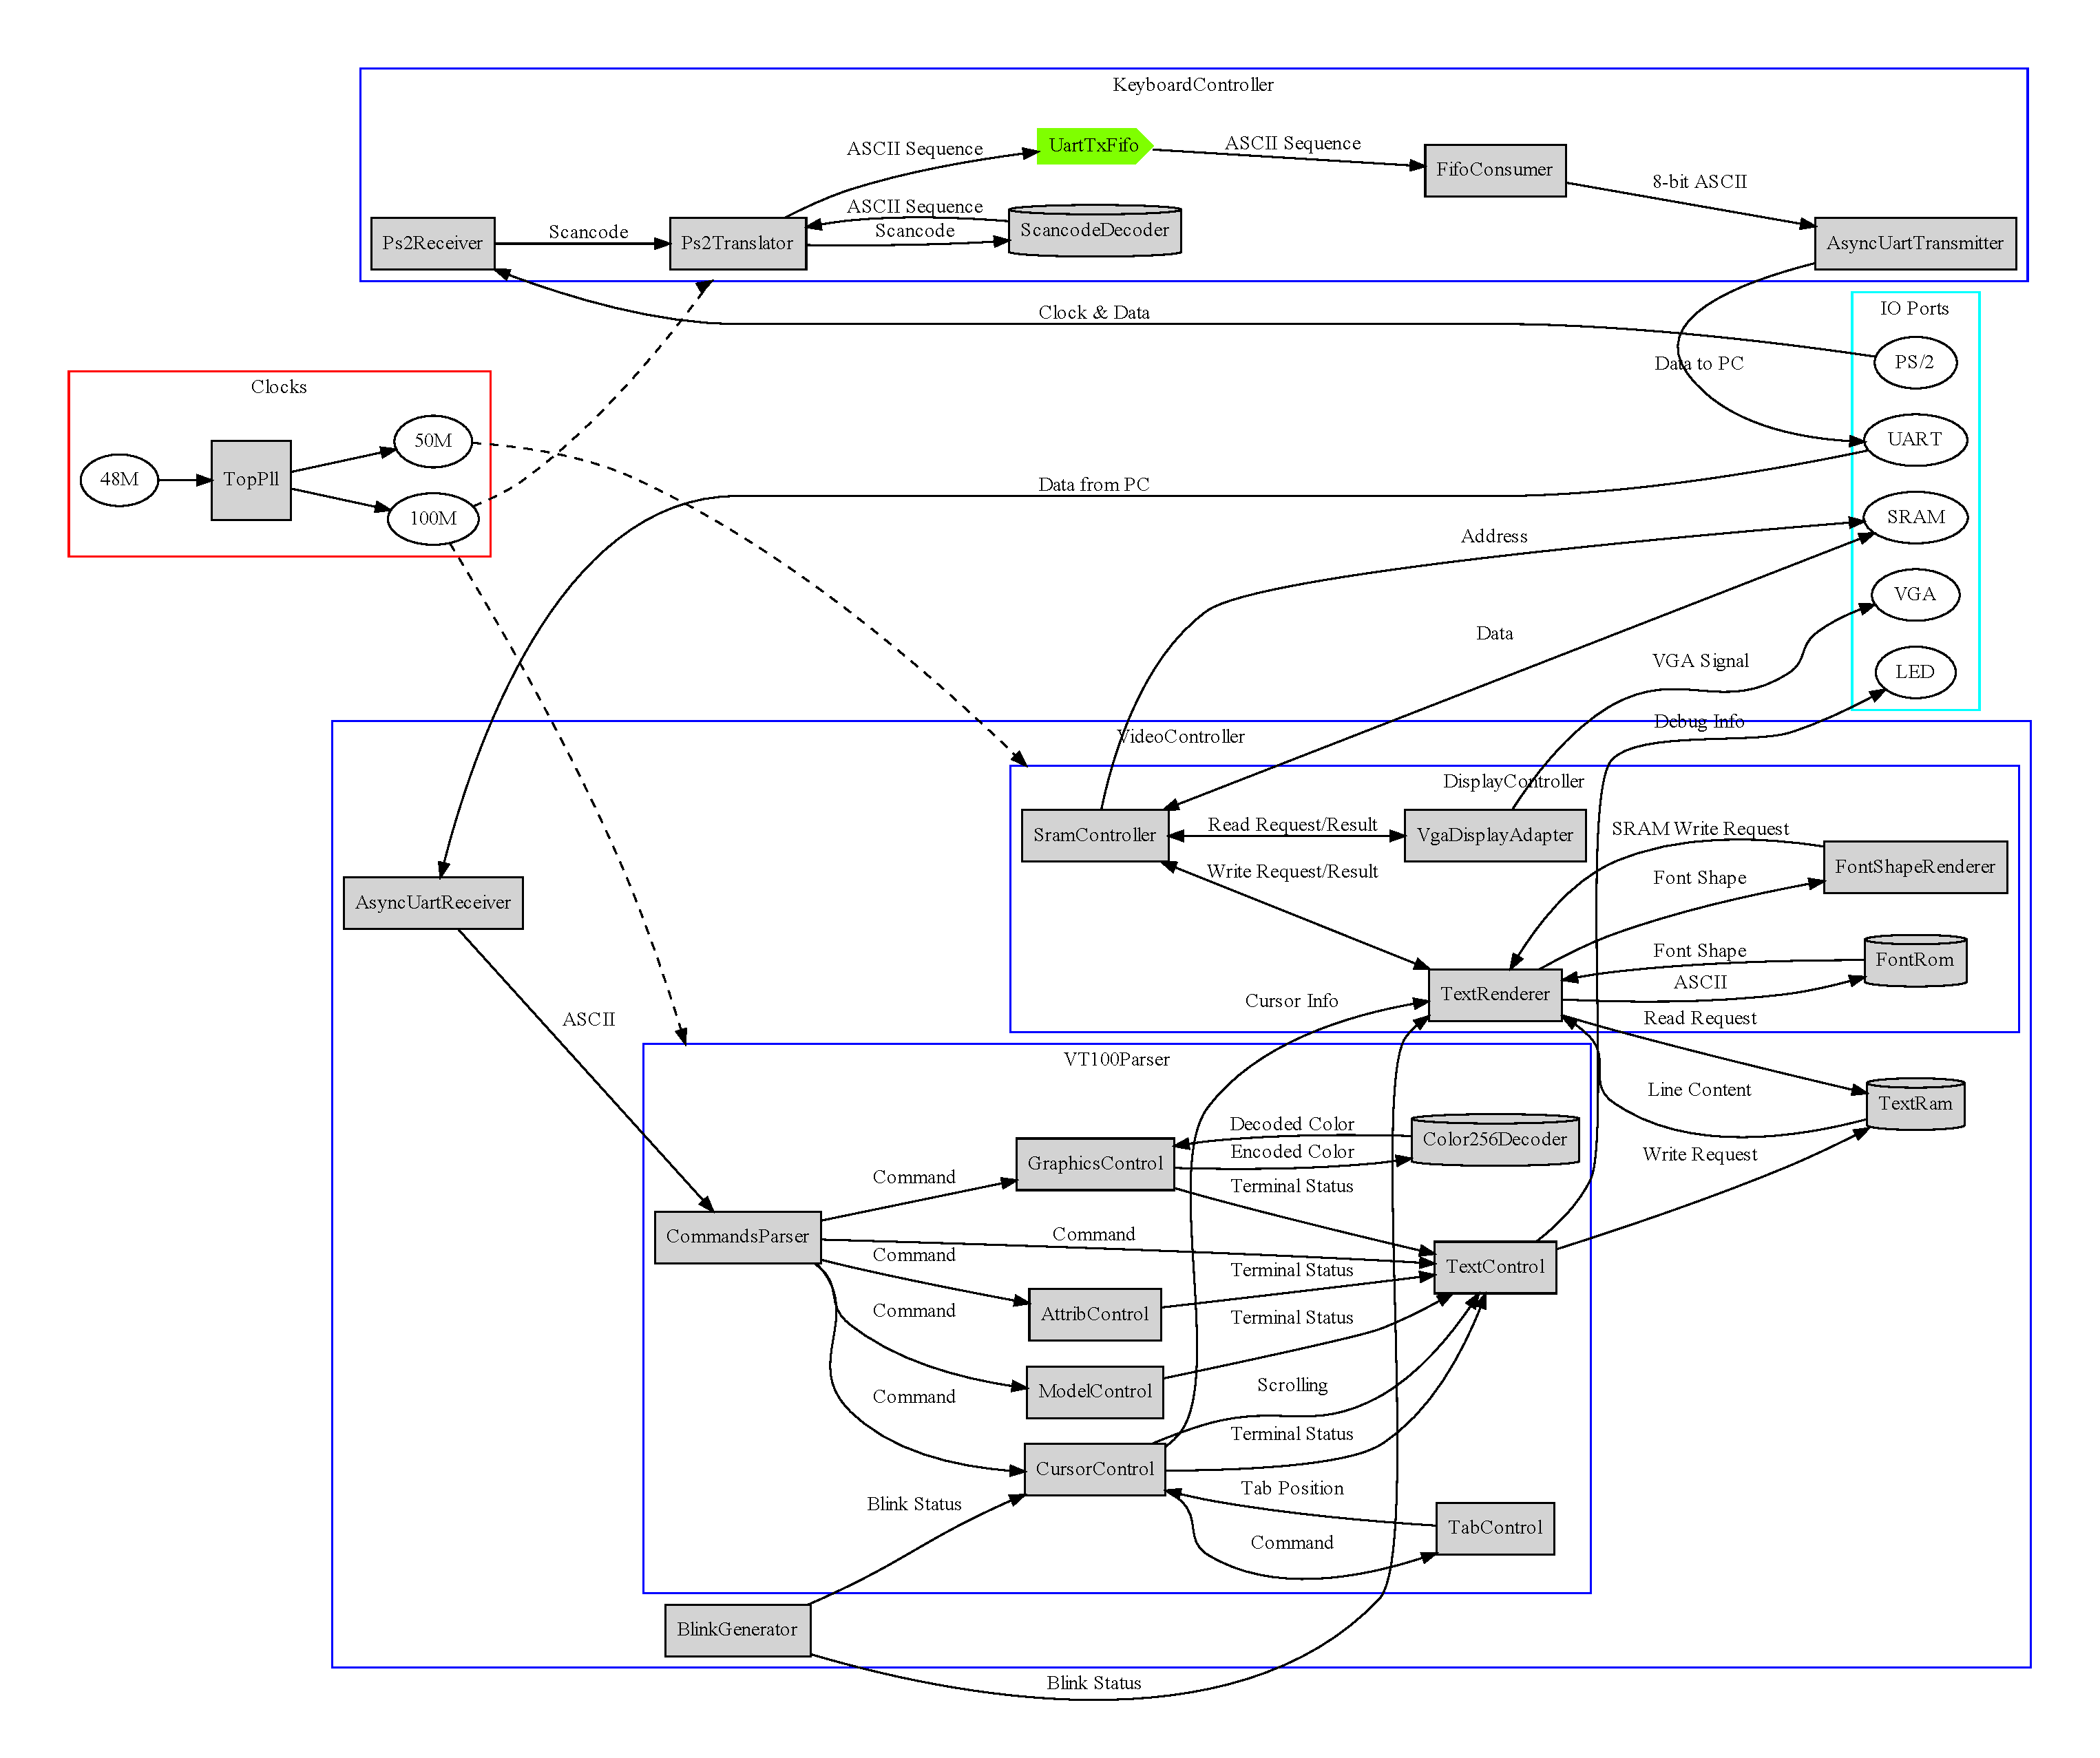
\includegraphics[width=\paperwidth]{architecture_final_dot.pdf}
}
\label{fig:final_architecture}
\caption{项目最终架构}
\end{figure}